\documentclass[journal,9pt]{IEEEtran}

\ifCLASSINFOpdf
\else
\fi
\usepackage{float}
\usepackage{url}
\usepackage{lettrine}
\usepackage{graphicx}
\usepackage[cmex10]{amsmath}
\usepackage{listings}
\usepackage{subfig}
\interdisplaylinepenalty=2500
\graphicspath{{img/}}
\usepackage[colorlinks=true,linkcolor=blue,citecolor=blue,urlcolor=blue]{hyperref}
\hyphenation{op-tical wire-less net-works}
\usepackage{newcent}

\begin{document}
\title{Odak: an open-source library for wave propagation and Fourier optics calculations}
\author{Kaan~Ak\c{s}it
\thanks{The author is with the Optical Microsystems Laboratory, Ko\c{c} University, Istanbul,
34450 TURKEY (e-mail: kaksit@ku.edu.tr).}}
\markboth{Optical Information Processing/ April~2011}
{Shell \MakeLowercase{\textit{et al.}}: Bare Demo of IEEEtran.cls
for the Journal of Optical Communications and Networking}
\IEEEpubid{0000--0000/00\$00.00~\copyright~2011 Optical Information Processing}


\maketitle
\begin{abstract}
This paper introduces an implementation of an open-source library implemented under Python programming language \cite{python} that provides built-in functions for wave propagation and Fourier optics calculation. Library provides callable functions for Fraunhofer diffraction and Fresnel diffraction under $odak.diffractions$ class. Library contains also a set of pre-defined aperture types under $odak.aperture$ class. In the near-future it is planned to implement a graphical user interface for end-user. Section \ref{section:justification} provides a justification of the implemented methods.
\end{abstract}
\begin{IEEEkeywords}
Beam propagation, Fourier optics, Fraunhofer diffraction, Fresnel diffraction, Python, Open-source.
\end{IEEEkeywords}
\IEEEpeerreviewmaketitle

\section{Introduction}
\label{section:introduction}
\lettrine{T}{here} are few optics simulation software available on the market and in the open-source world. One of the most known optics simulation software on the market is ZEMAX \cite{zemax}. In open-source world there are also quality software such as Opus \cite{opus}. The full list of available optics simulation programs can be found under \cite{optalix}. The aim of this project is to provide an optics alternative simulation software. With such an alternative, it will be a lot more easier to implement wave propagation and Fourier optics inside a Python script, thus easiness is provided to Python users. Python is the most preferred programming language for academical purposes beside MATLAB and Octave. Syntaxes of Python is similar in a sense to ones in MATLAB and also provides far more better code flow control. It is also aimed to provide a licence free work bench for different platforms (currently supports only on Linux and Microsoft Windows).

The introduced system in this paper is able to provide calculations for Fourier calculations. But in near future a ray tracing extension with a graphical user interface and ray-tracing ability will be provided to the end-users.

\section{How to make it work}
\label{section:howtomakeitwork}
\subsection{Under Linux}
Once $sample.py$ and $odak.py$ are downloaded from \cite{odak} and saved under the same folder; Linux users can download the dependencies of $matplotlib$, $numpy$ and $SciPy$ from their default package managers and they can execute the $sample.py$ using $python~sample.py$ command under the terminal. Note that running this script will show you the results of the sample questions in Section \ref{section:justification}.
\subsection{Under Microsoft Windows}
Windows packages of Python 2.7 from \cite{python}, $numpy$ from \cite{numpy}, $SciPy$ from \cite{scipy} and $matplotlib$ from \cite{matplotlib} should be downloaded and installed in the targeted computer. Once $sample.py$ and $odak.py$ are downloaded from \cite{odak} and saved under the same folder; double clicking on $sample.py$ will directly run or open an Idle window, if Idle window is opened simply press run (F5) from the above menus of the Idle. Note that running this script will show you the results of the sample questions in Section \ref{section:justification}.

\section{Manual}
\label{section:manual}

This parts describes available functions inside the library described in this paper.
\subsection{Class:odak.aperture}
This class contains pre-defined apertures. Currently available callable aperture function are as in Table \ref{table:aperture}.

\begin{tabular}{ l }
  \\Available callable aperture functions\\ \hline
  $odak.aperture.circle()$\\
  $odak.aperture.lens()$\\
  $odak.aperture.rectangle()$\\
  $odak.aperture.sinamgrating()$\\
  $odak.aperture.twoslits()$\\
\label{table:aperture}
\end{tabular}

Figure \ref{fig:aperture} shows different available apertures from $odak.aperture$ class.

\begin{figure}[H]
  \centering
  \subfloat[$odak.aperture.circle()$.]{\label{fig:circle}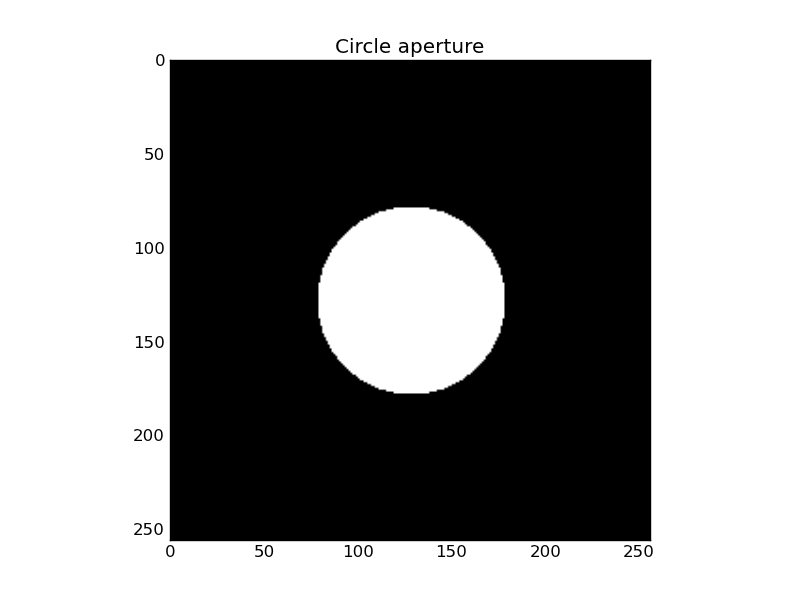
\includegraphics[width=0.23\textwidth]{circle}} \hspace{2mm}   
  \subfloat[$odak.aperture.rectangle()$.]{\label{fig:rectangle}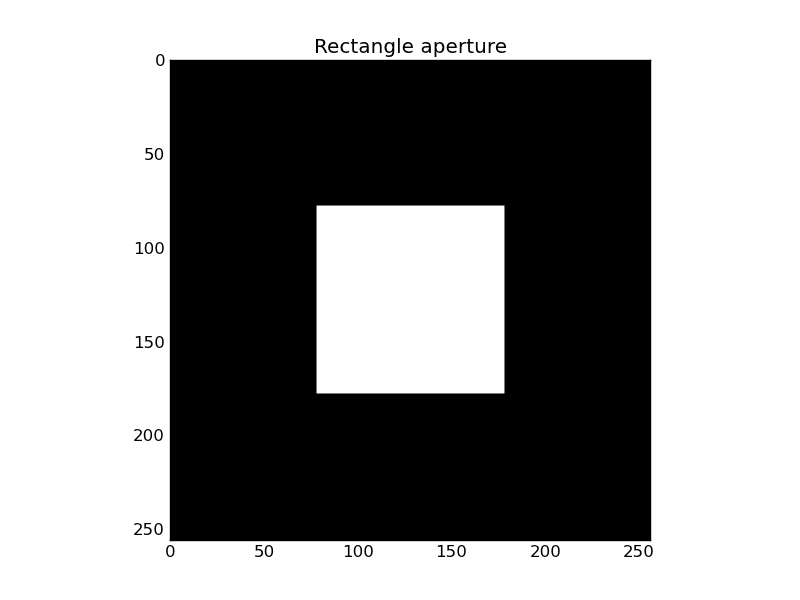
\includegraphics[width=0.23\textwidth]{rectangle}} \hspace{2mm}       
  \subfloat[$odak.aperture.twoslits()$.]{\label{fig:twoslits}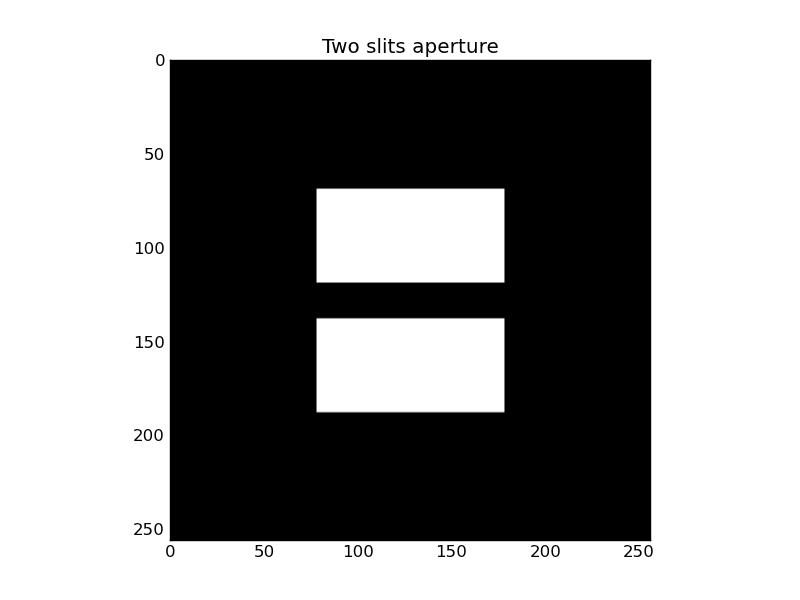
\includegraphics[width=0.23\textwidth]{twoslits}} \hspace{2mm}    
  \subfloat[$odak.aperture.sinamgrating()$.]{\label{fig:sinamgrating}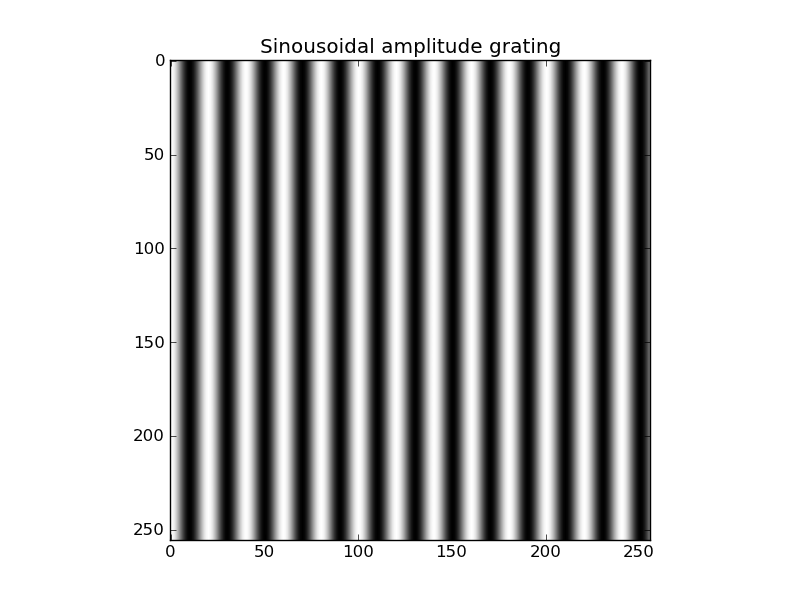
\includegraphics[width=0.23\textwidth]{sinamgrating}} \hspace{2mm}   
  \caption{Sample apertures.}
  \label{fig:aperture}  
\end{figure}
\IEEEpubidadjcol

Explanation of each function is given in subsections provided in below. Note that each variable corresponds to a single element or a pixel in the created aperture array.\\

\subsubsection{odak.aperture.circle(nx,ny,radius)}
nx defines the width of the whole aperture. ny defines the height of the whole aperture. radius defines the radius of the white region.\\
\subsubsection{odak.aperture.lens(self,nx,ny,focal,wavelength)}
nx defines the width of the whole aperture. ny defines the height of the whole aperture. focal is the focal length in meters of the lens. Wavelength is the wavelength in meters of the input light.\\
\subsubsection{odak.aperture.rectangle(nx,ny,side)}
nx defines the width of the whole aperture. ny defines the height of the whole aperture. side defines one side of the white region.\\
\subsubsection{odak.aperture.sinamgrating(self,nx,ny,grating)}
nx defines the width of the whole aperture. ny defines the height of the whole aperture. Grating is the spatial period in pixels.\\
\subsubsection{odak.aperture.twoslits(nx,ny,X,Y,delta)}
nx defines the width of the whole aperture. ny defines the height of the whole aperture.  X defines the width of the each rectangle shaped white region. Y defines the height of the each rectangle shaped white region. delta is the distance between the centroids of the two white rectangle regions.\\

\subsection{Class:odak.diffractions}
This class contains pre-defined callable functions for Fraunhofer and Fresnel diffractions. Currently available callable built-in functions inside $odak.diffractions$ are as in Table \ref{table:diffractions}.

\begin{tabular}{ l }
  \\Available callable aperture functions\\ \hline
  $odak.diffractions.fresnelfraunhofer()$\\
  $odak.diffractions.fraunhoferintegral()$\\
  $odak.diffractions.count()$\\
  $odak.diffractions.talbotcalculate()$\\
\label{table:diffractions}
\end{tabular}

\subsubsection{odak.diffractions.fresnelfraunhofer(obj,wavelength,distance)}
obj here is an numpy array. wavelength is the wavelength in nano-meters of the input light. Distance here is the distance in meters between the object and the desired plane. This function computes Fraunhofer diffraction of a given input\\
\subsubsection{odak.diffractions.fraunhoferintegral(obj)}
obj here is an numpy array. This function computes 1D FFT of the given 2D array. \\
\subsubsection{odak.diffractions.count(obj,x)}
obj here is an numpy array. This function computes how many x is available inside obj array. \\
\subsubsection{odak.diffractions.talbotcalculate(obj,grating,wavelength)}
grating is the spatial period in meters of the diffraction grating. Wavelength is the wavelength in meters of the incoming light. \\

\section{Justification}
\label{section:justification}

\subsection{Implementation of Fresnel/Fraunhofer diffraction}

Fraunhofer diffraction occurs when the statement in Equation \ref{equ:fraunhoferstatement}. Fresnel diffraction occurs when the statement in Equation \ref{equ:fresnelstatement}.

\begin{equation}
\label{equ:fraunhoferstatement}
\begin{split}
F=\frac{a^2}{L \lambda}<<1
\end{split}
\end{equation}

\begin{equation}
\label{equ:fresnelstatement}
\begin{split}
F = \frac{a^2}{L\lambda} \ge 1 
\end{split}
\end{equation}

Once this condition is fulfilled far-field approximation of Fraunhofer is presented as in Equation \ref{equ:fraunhofer}. Fresnel is represented by Equation \ref{equ:fresnel}, Equation \ref{equ:r} and Equation \ref{equ:k}.

\begin{equation}
\label{equ:fraunhofer}
\begin{split}
U(x,y)=\frac{e^{ikz}e^{\frac{ik(x^2+y^2)}{2z}}}{i\lambda z}\int\int_{-\infty}^{\infty}u(x',y')\\
e^{-i\frac{2\pi}{\lambda z}(x'x+y'y)}dx'dy'
\end{split}
\end{equation}

\begin{equation}
\label{equ:fresnel}
\begin{split}
E(x,y,z)={z \over {i \lambda}} \iint_{-\infty}^{+\infty}{ E(x',y',0) \frac{e^{ikr}}{r^2}}dx'dy' 
\end{split}
\end{equation}

\begin{equation}
\label{equ:r}
\begin{split}
r=\sqrt{(x-x')^2+(y-y')^2+z^2}
\end{split}
\end{equation}

\begin{equation}
\label{equ:k}
\begin{split}
k = { 2 \pi \over \lambda }
\end{split}
\end{equation}


Similar to Fourier transform and Equation \ref{equ:fraunhofer} and Equation \ref{equ:fresnel} contains an integral. Analytical solution of this integral is impossible for all but the simplest diffraction geometries. Therefore, it is usually calculated numerically. The integral can be solved as in discrete Fourier transform algorithms. For this purpose $Cooley-Tukey$ algorithm is employed. An implementation of $Cooley-Tukey$ algorithm as in \cite{cooleytukey} is made and shown in below code, Equation \ref{equ:cooleytukey} is employed for the implementation. Beside this implementation, built-in $fft2$ command is also applicable.

\lstset{language=Python,breaklines=true}
\lstinputlisting[language=Python,firstline=69,lastline=75]{../source/lib/odak.py}

\begin{equation}
\label{equ:cooleytukey}
\begin{split}
\begin{matrix} X_k= \underbrace{\sum \limits_{m=0}^{N/2-1} x_{2m}   e^{-\frac{2\pi i}{N/2} mk}}_{\mathrm{DFT\;of\;even-indexed\;part\;of\;} x_m} {} \\
+  e^{-\frac{2\pi i}{N}k}
 \underbrace{\sum \limits_{m=0}^{N/2-1} x_{2m+1} e^{-\frac{2\pi i}{N/2} mk}}_{\mathrm{DFT\;of\;odd-indexed\;part\;of\;} x_m} \\
 =  E_k + e^{-\frac{2\pi i}{N}k} O_k.
\end{matrix}
\end{split}
\end{equation}

After the implementation of the $fraunhoferintegral$ function or in other saying 1D DFT algorithm with a 2D input; using the flow chart in Figure \ref{fig:cooleytukey}, Equation \ref{equ:fraunhofer} is implemented as in below code. Implementation is made using fft approach.

\lstset{language=Python,breaklines=true}
\lstinputlisting[language=Python,firstline=51,lastline=68]{../source/lib/odak.py}

\begin{figure}[H]
\centering
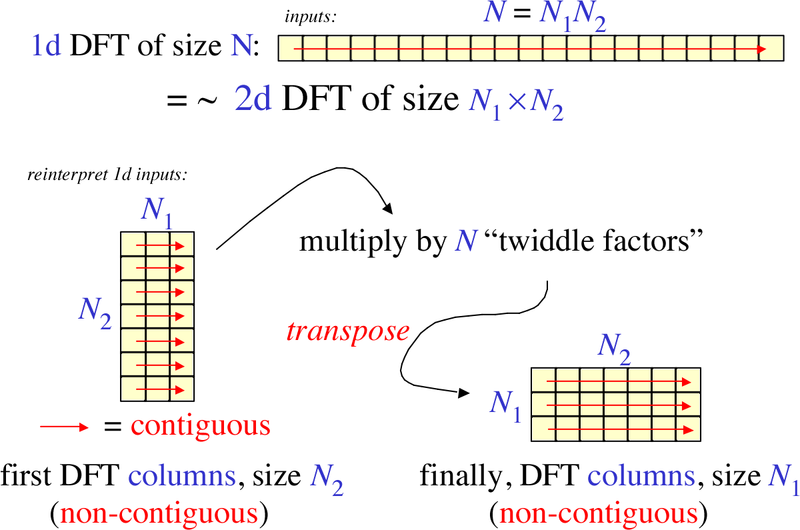
\includegraphics[width=2.7in]{cooleytukey}
\caption{Way to implement Fraunhofer integral, \cite{cooleytukey}.}
\label{fig:cooleytukey}
\end{figure}

\subsection{Sample question I}
Sample question I is as follows: Starting with a rectangular aperture of size 1mm, observe the diffraction pattern at different critical propagation distances.

Rectangular aperture with size of 1mm can be examined under Figure \ref{fig:rectangle1m}. For the rest of the calculations wavelength is chosen as $532$nm. Below code is used to plot the diffraction patterns at different critical propagation distances.

\lstset{language=Python,breaklines=true}
\lstinputlisting[language=Python,firstline=11,lastline=28]{../source/lib/sample.py}

\begin{figure}[H]
\centering
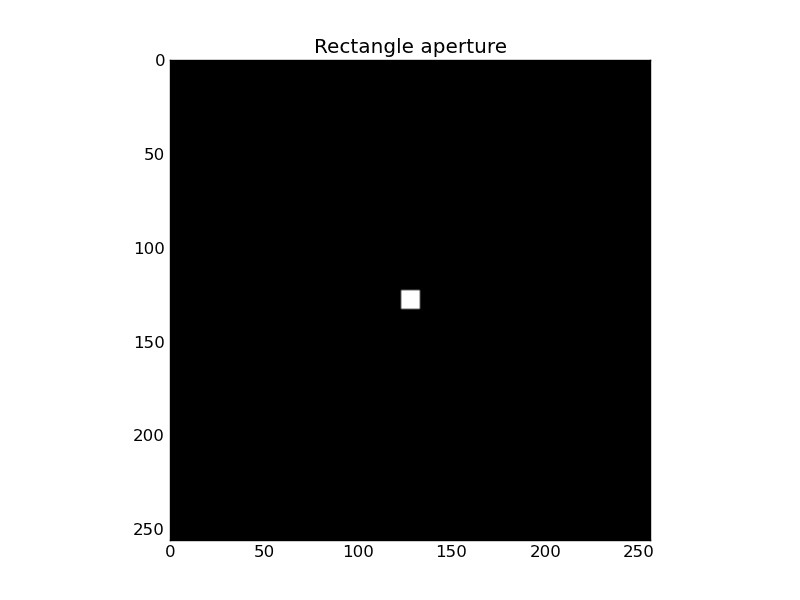
\includegraphics[width=2.3in]{rectangle1mm}
\caption{Rectangular aperture with size of 1mm. Here 10 pixel corresponds to 1mm.}
\label{fig:rectangle1m}
\end{figure}

\subsubsection{Fresnel/Fraunhofer diffraction patterns at different distances for sample question I}

Distances of each Fraunhofer diffraction pattern is written on top of the figures. After each figure an intensity profile is provided as the next figure.
\begin{figure}[H]
\centering
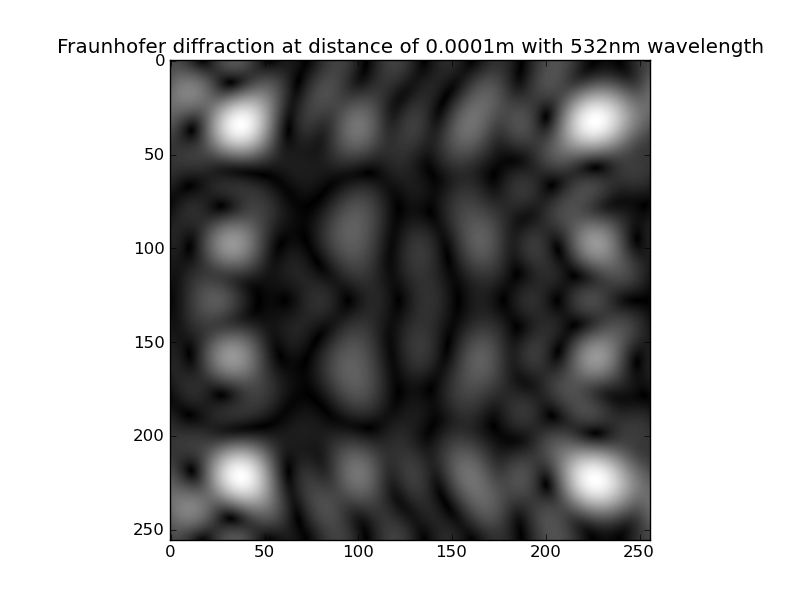
\includegraphics[width=1.9in]{q1d100um}
\caption{Fraunhofer diffraction pattern}
\label{fig:q1d100um}
\end{figure}

\begin{figure}[H]
\centering
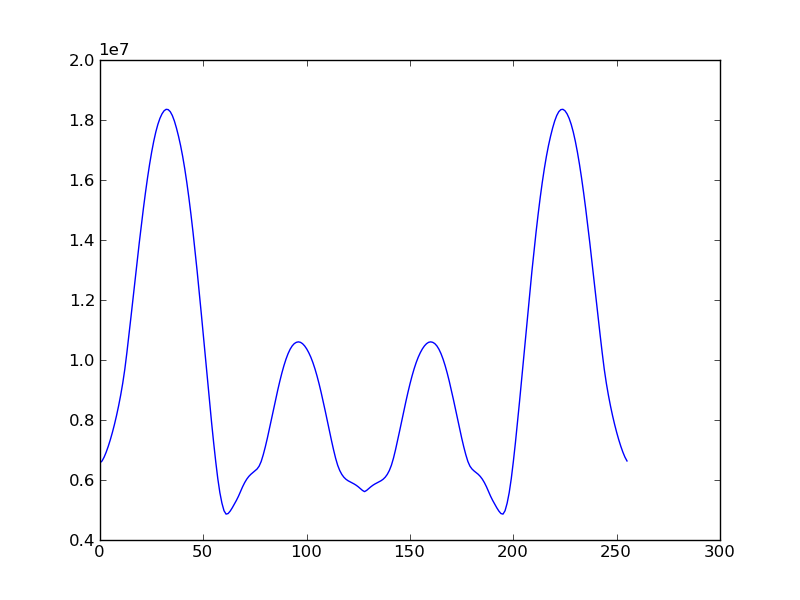
\includegraphics[width=1.9in]{q1i100um}
\caption{Intensity profile of Fraunhofer diffraction pattern}
\label{fig:q1i100um}
\end{figure}

\begin{figure}[H]
\centering
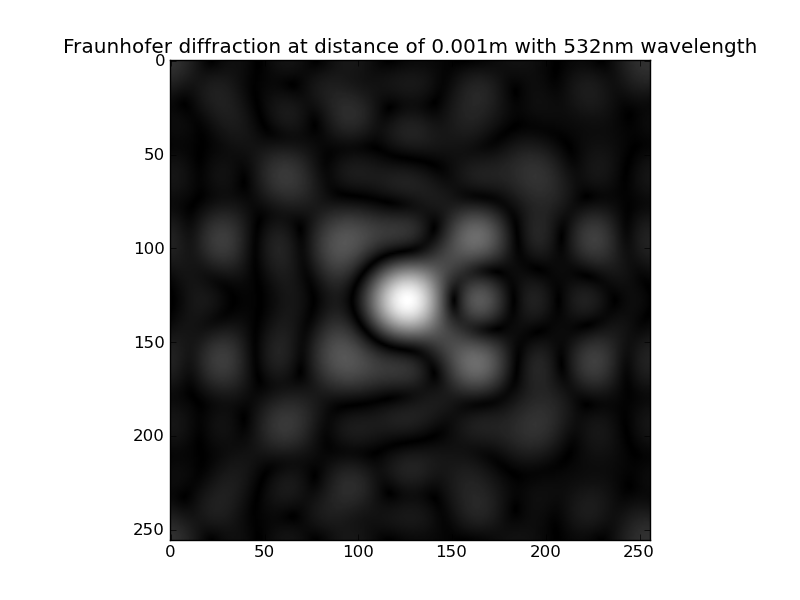
\includegraphics[width=1.9in]{q1d1mm}
\caption{Fraunhofer diffraction pattern}
\label{fig:q1d1mm}
\end{figure}

\begin{figure}[H]
\centering
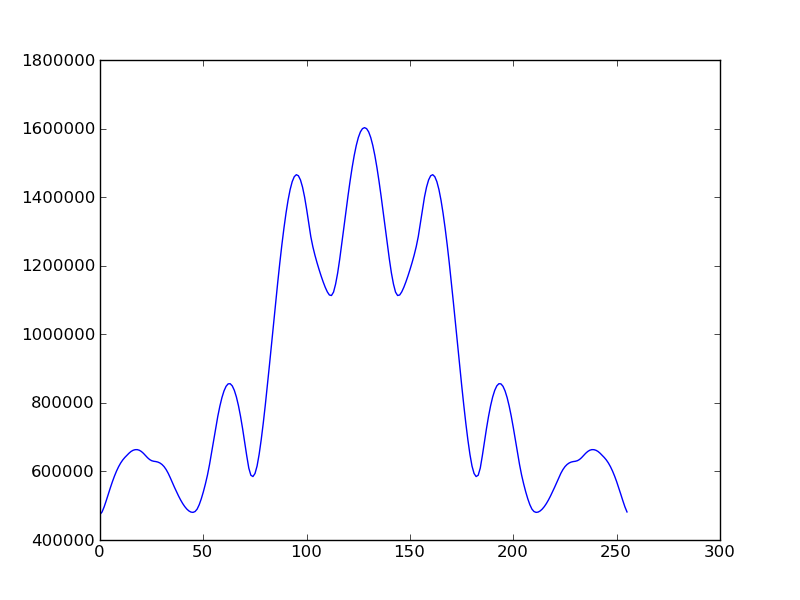
\includegraphics[width=1.9in]{q1i1mm}
\caption{Intensity profile of Fraunhofer diffraction pattern}
\label{fig:q1i1mm}
\end{figure}

\begin{figure}[H]
\centering
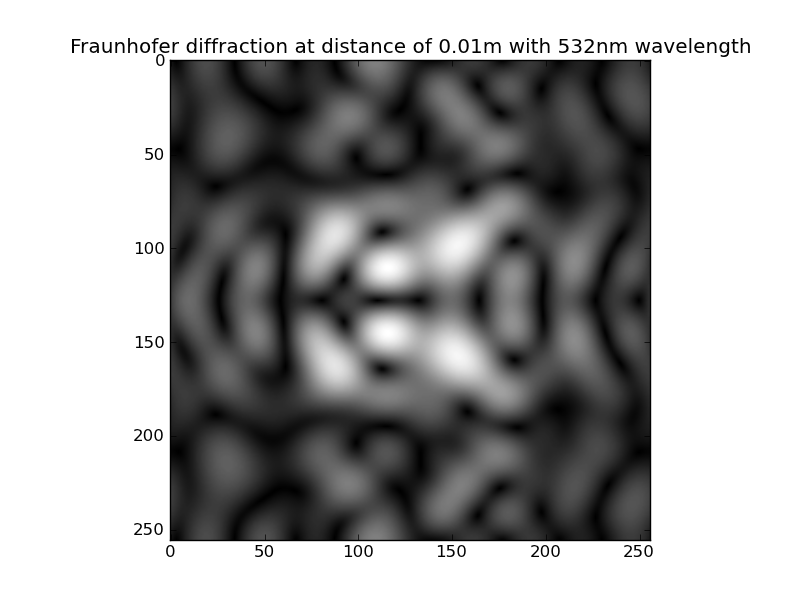
\includegraphics[width=1.9in]{q1d10mm}
\caption{Fraunhofer diffraction pattern}
\label{fig:q1d10mm}
\end{figure}

\begin{figure}[H]
\centering
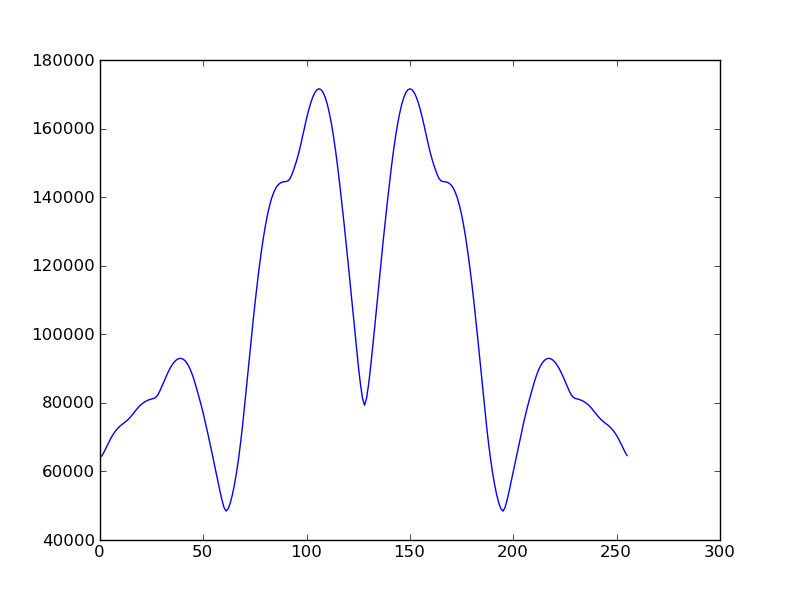
\includegraphics[width=1.9in]{q1i10mm}
\caption{Intensity profile of Fraunhofer diffraction pattern}
\label{fig:q1i10mm}
\end{figure}

\begin{figure}[H]
\centering
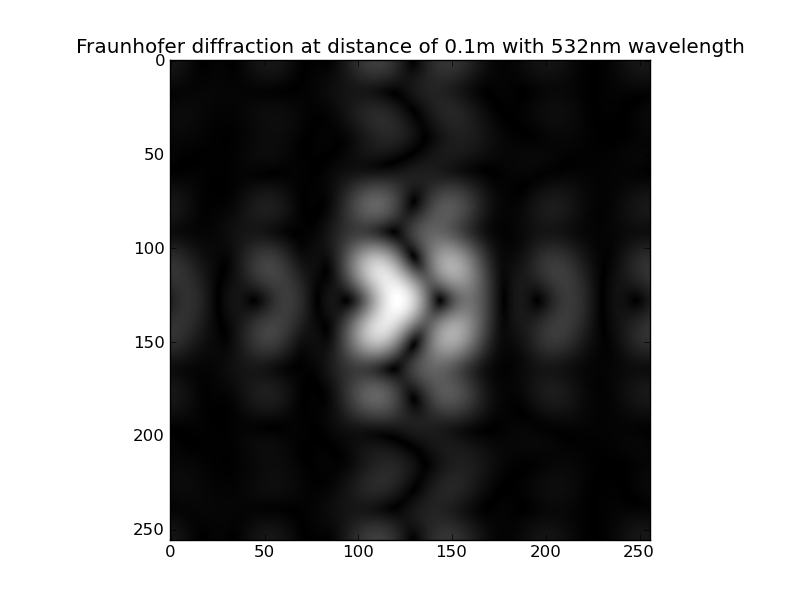
\includegraphics[width=1.9in]{q1d100mm}
\caption{Fraunhofer diffraction pattern}
\label{fig:q1d100mm}
\end{figure}

\begin{figure}[H]
\centering
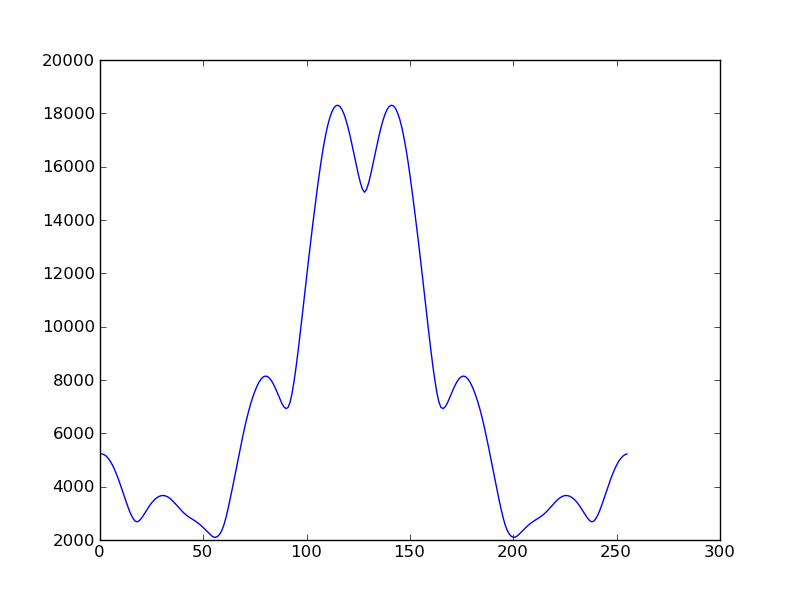
\includegraphics[width=1.9in]{q1i100mm}
\caption{Intensity profile of Fraunhofer diffraction pattern at $0.1$m distance}
\label{fig:q1i100mm}
\end{figure}

\begin{figure}[H]
\centering
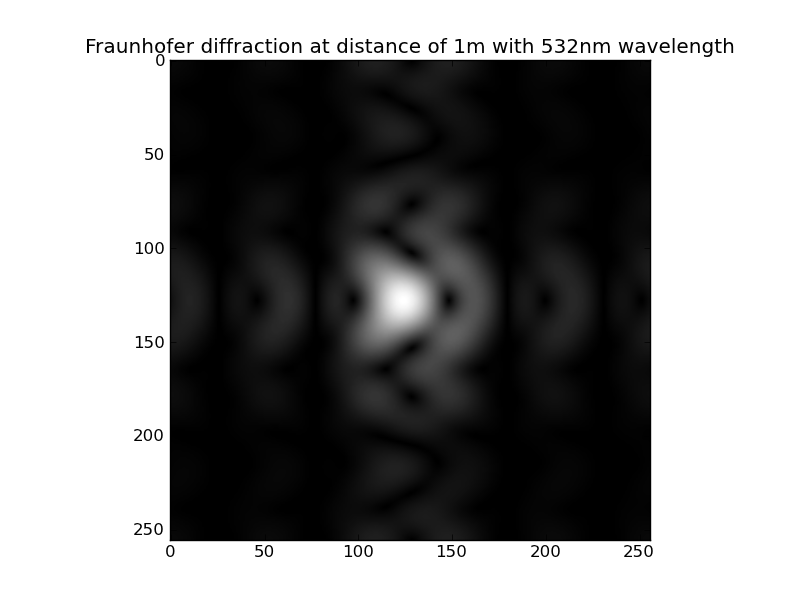
\includegraphics[width=1.9in]{q1d1m}
\caption{Fraunhofer diffraction pattern at $1$m distance}
\label{fig:q1d1m}
\end{figure}

\begin{figure}[H]
\centering
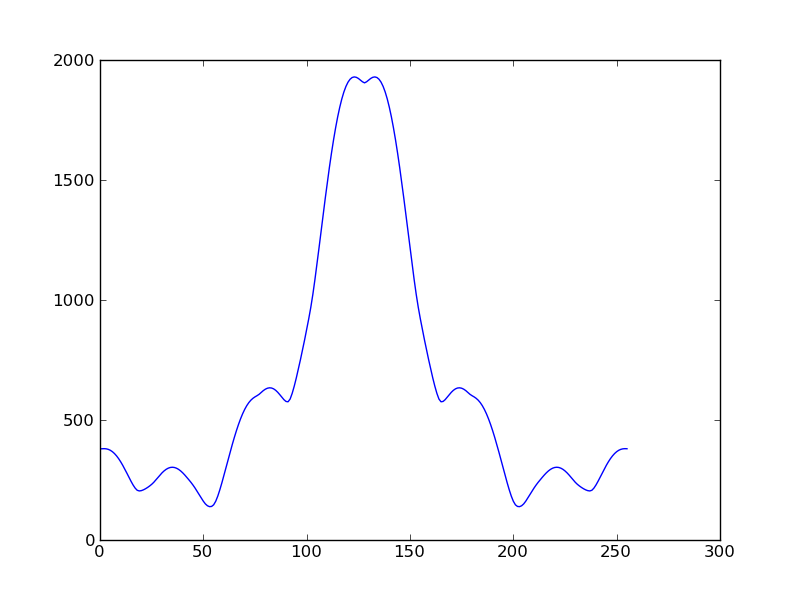
\includegraphics[width=1.9in]{q1i1m}
\caption{Intensity profile of Fraunhofer diffraction pattern}
\label{fig:q1i1m}
\end{figure}

\begin{figure}[H]
\centering
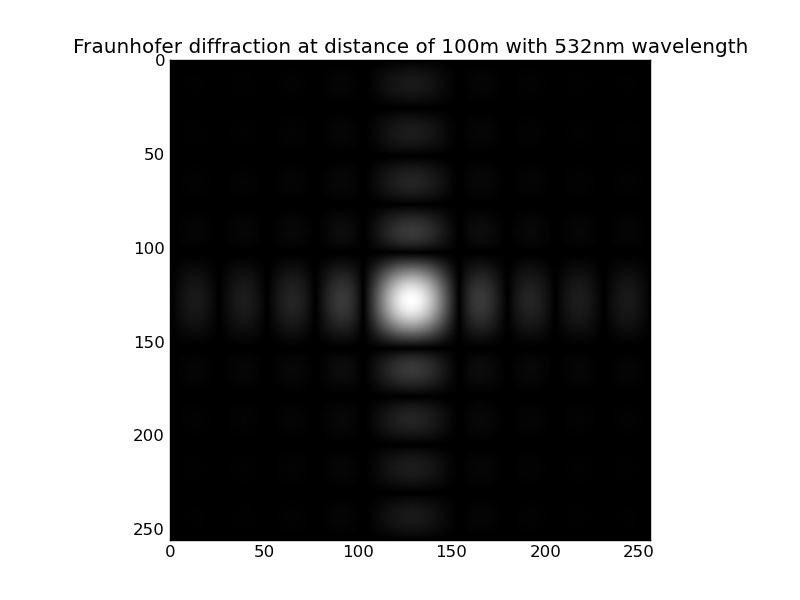
\includegraphics[width=1.9in]{q1d100m}
\caption{Fraunhofer diffraction pattern at $100$m distance}
\label{fig:q1d100m}
\end{figure}

\begin{figure}[H]
\centering
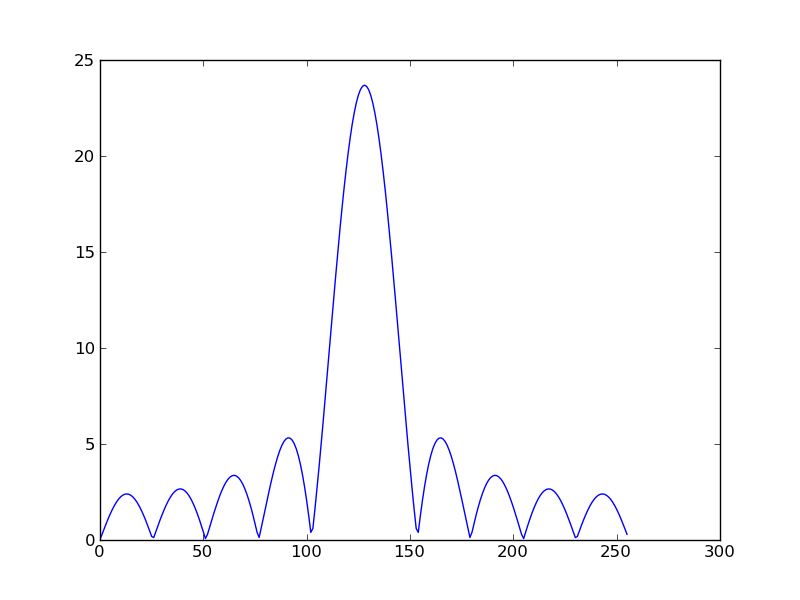
\includegraphics[width=1.9in]{q1i100m}
\caption{Intensity profile of Fraunhofer diffraction pattern}
\label{fig:q1i100m}
\end{figure}

\subsection{Sample question II}
Sample question II is as follows: Assume a converging spherical beam illuminates an object pattern of your choice (let's say a triangular or rectangular shaped binary object). Assume the object size is $1$mm and the spherical wave is converging to a point $15$mm behind the object. Find the irradiance profile at the focus of the spherical wave ($15$mm away from the object) and also at $30$mm away from the object. Briefly explain what you observe.

Same aperture as in Figure \ref{fig:rectangle1m} is used during the solution of this sample question. To focus the beam a lens is employed at the right position with the focal length of $15$m. Lens transmittance function is calculated by implemented function called $odak.aperture.lens()$, see Figure \ref{fig:lenstrans} for lens transmittance function.

\lstset{language=Python,breaklines=true}
\lstinputlisting[language=Python,firstline=11,lastline=28]{../source/lib/sample.py}

\begin{figure}[H]
\centering
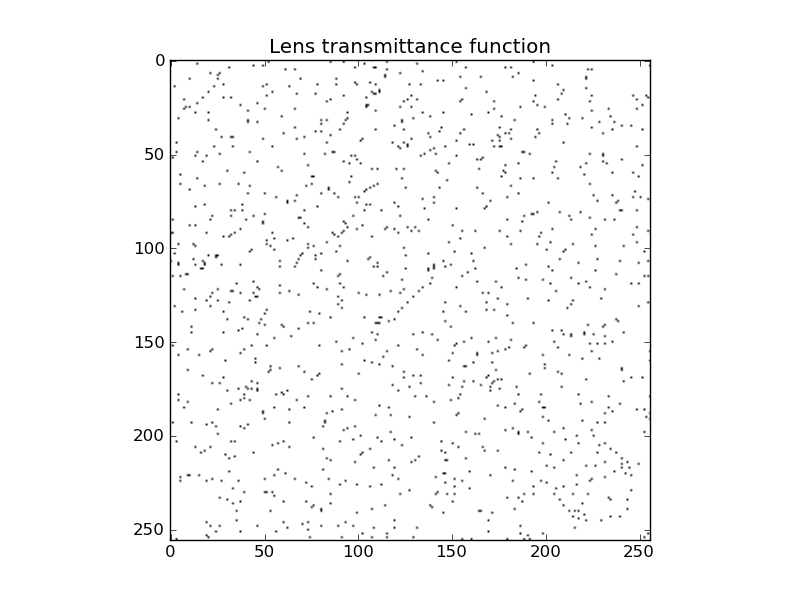
\includegraphics[width=1.9in]{lenstrans}
\caption{Lens transmittance function.}
\label{fig:lenstrans}
\end{figure}


Here are the outputs of the diffraction pattern under different distances:

\begin{figure}[H]
\centering
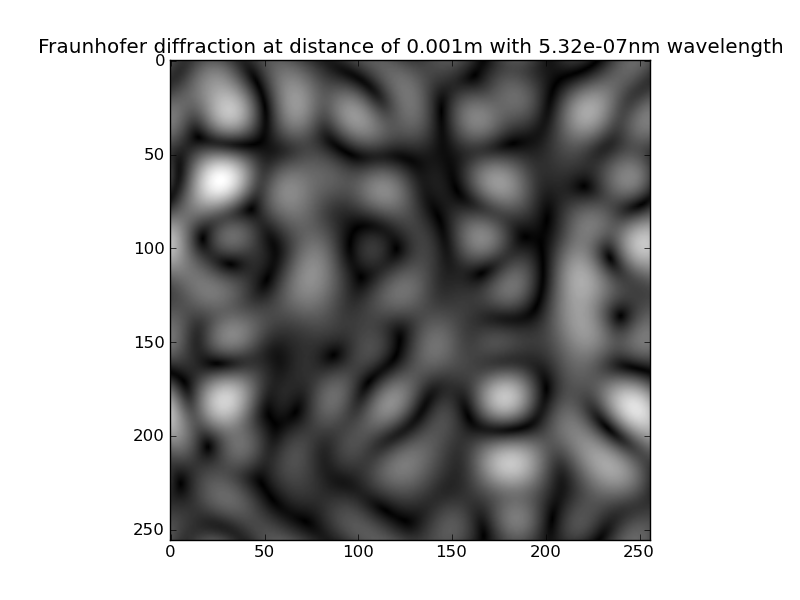
\includegraphics[width=1.9in]{q2d1mm}
\caption{Diffraction pattern.}
\label{fig:q2d1mm}
\end{figure}

\begin{figure}[H]
\centering
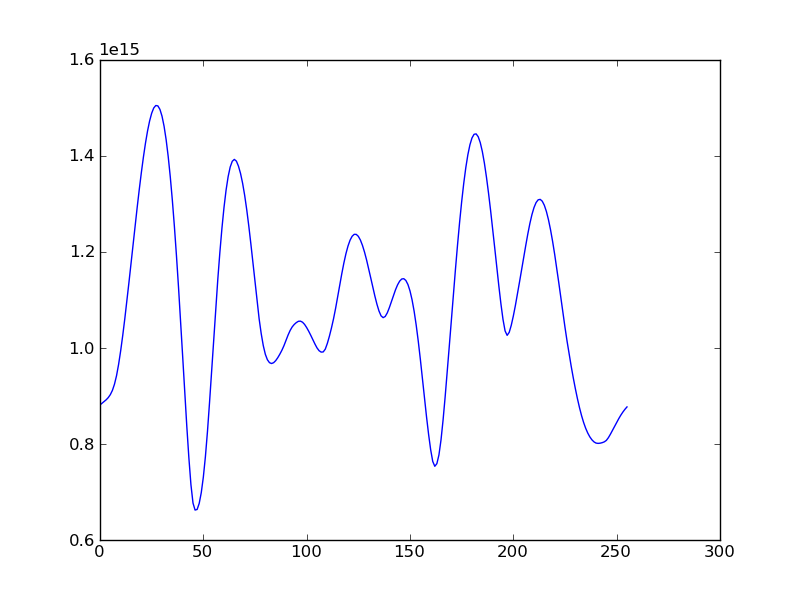
\includegraphics[width=1.9in]{q2s1mm}
\caption{Diffraction pattern cross-section.}
\label{fig:q2s1mm}
\end{figure}

\begin{figure}[H]
\centering
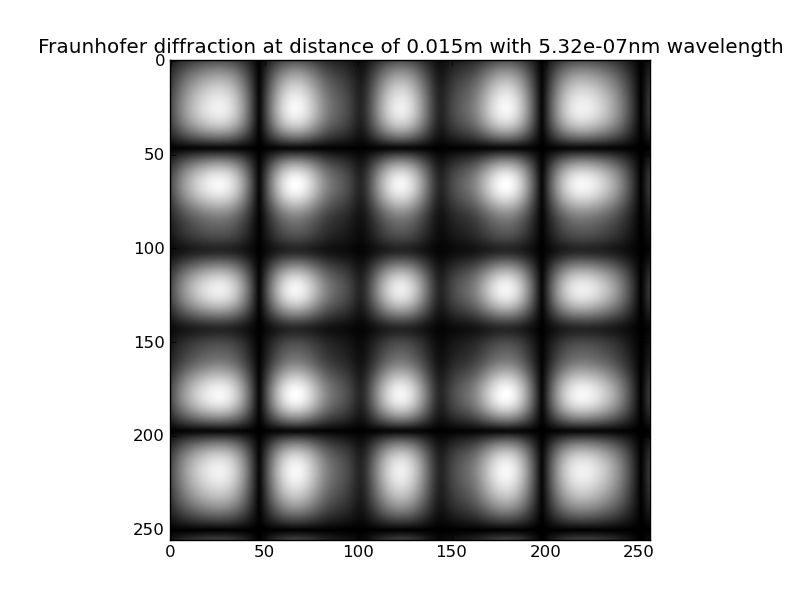
\includegraphics[width=1.9in]{q2d15mm}
\caption{Diffraction pattern.}
\label{fig:q2d15mm}
\end{figure}

\begin{figure}[H]
\centering
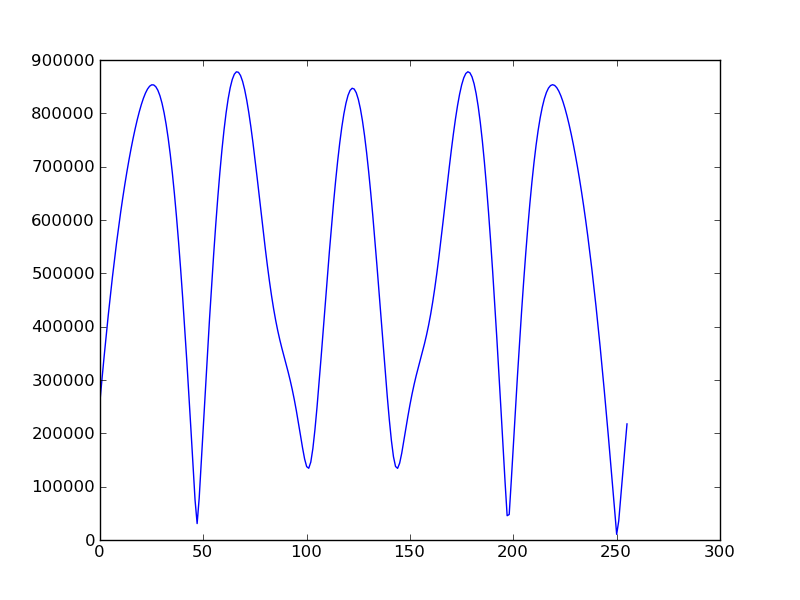
\includegraphics[width=1.9in]{q2s15mm}
\caption{Diffraction pattern cross-section.}
\label{fig:q2s15mm}
\end{figure}

\begin{figure}[H]
\centering
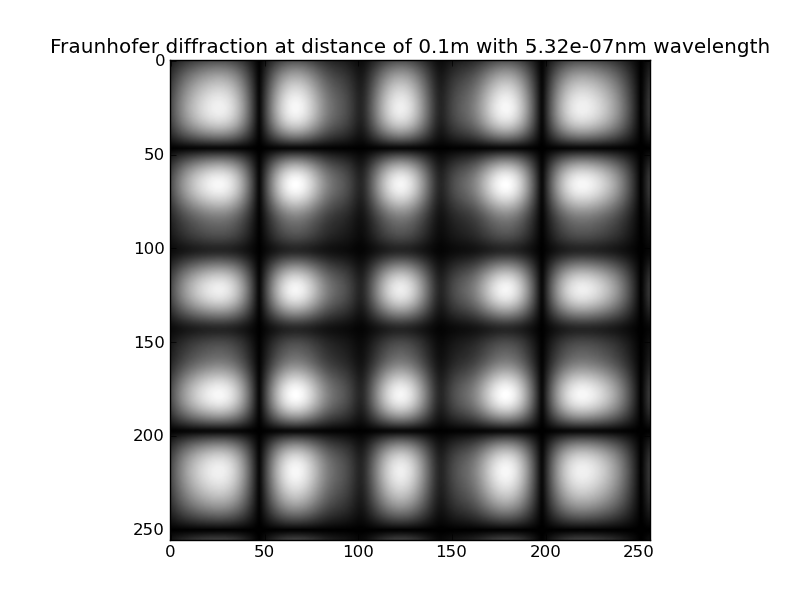
\includegraphics[width=1.9in]{q2d100mm}
\caption{Diffraction pattern.}
\label{fig:q2d100mm}
\end{figure}

\begin{figure}[H]
\centering
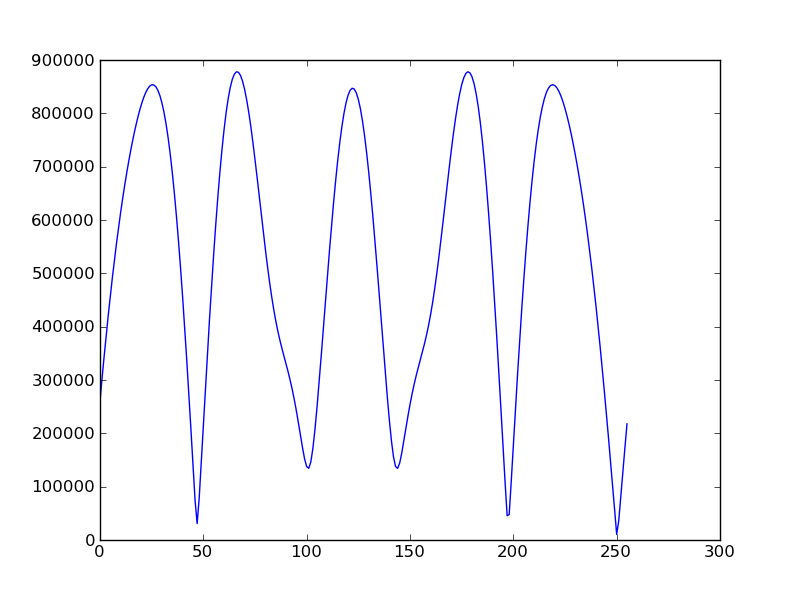
\includegraphics[width=1.9in]{q2s100mm}
\caption{Diffraction pattern cross-section.}
\label{fig:q2s100mm}
\end{figure}

\subsection{Sample question III}
 Observe the diffraction patterns after sinusoidal amplitude grating at different critical propagation distances (e.g. at different Talbot images). Comment on the results.

Talbot distance is calculated using Equation \ref{equ:talbot}. For $\lambda=532$nm and $\Lambda=2~10^{-7}$um. As discussed in \cite{goodman2005introduction}, a rectangular aperture is multiplied with Equation \ref{equ:sinam} to form a sinusoidal amplitude grating.

\begin{equation}
\label{equ:talbot}
\begin{split}
T=\frac{2\Lambda^2}{\lambda}
\end{split}
\end{equation}


\begin{equation}
\label{equ:sinam}
\begin{split}
t_A(x,y)=\frac{1}{2}+\frac{1}{2}\cos(2\pi x\frac{1}{\Lambda})
\end{split}
\end{equation}

After multiplying the rectangle form Figure \ref{fig:sinam} is derived.

\begin{figure}[H]
\centering
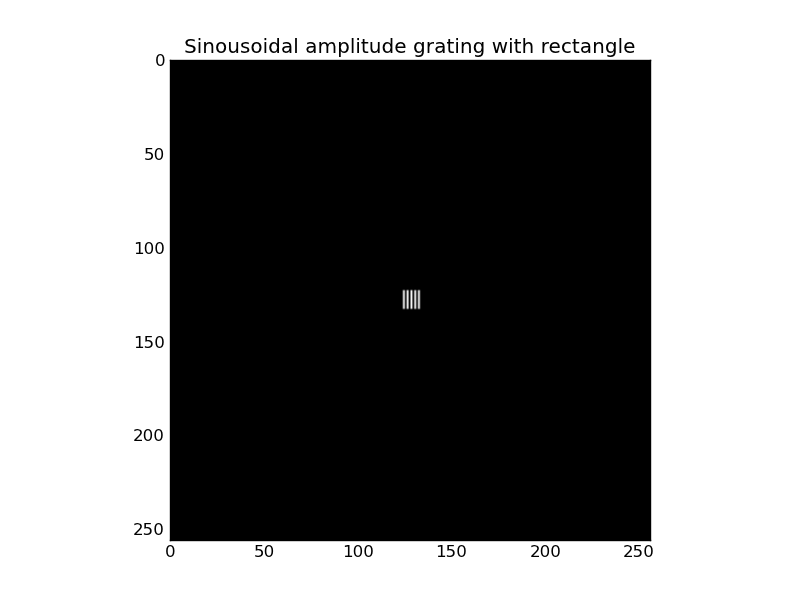
\includegraphics[width=1.9in]{sinam}
\caption{Derived sinusoidal amplitude grating.}
\label{fig:sinam}
\end{figure}

Below code is used to compute the sample question III.
\lstset{language=Python,breaklines=true}
\lstinputlisting[language=Python,firstline=30,lastline=49]{../source/lib/sample.py}

In different Talbot distances below Figures are derived using the above code.

\begin{figure}[H]
\centering
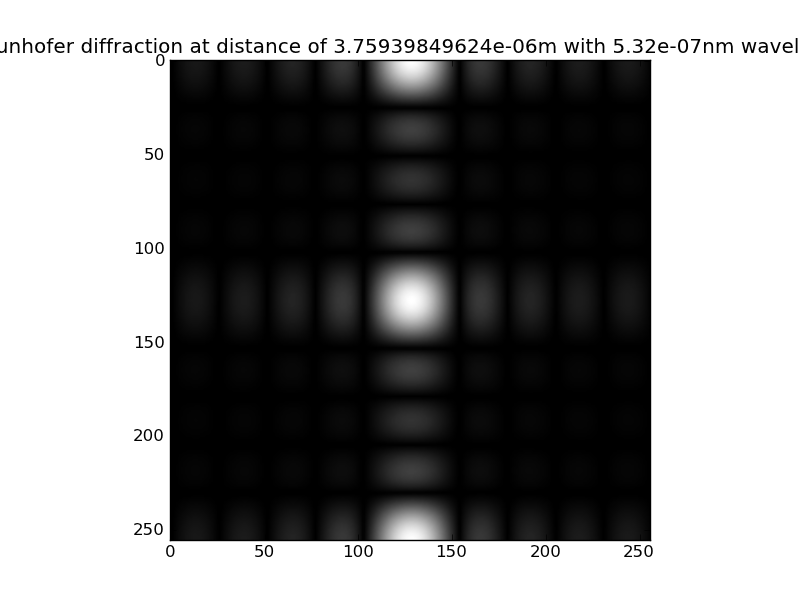
\includegraphics[width=1.9in]{q3d1}
\caption{Derived sinusoidal amplitude grating diffraction pattern.}
\label{fig:q3d1}
\end{figure}

\begin{figure}[H]
\centering
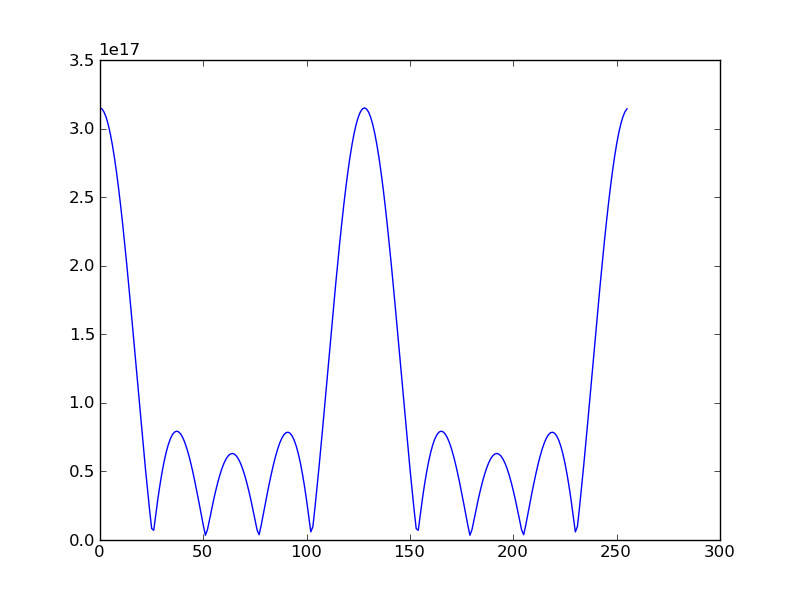
\includegraphics[width=1.9in]{q3s1}
\caption{Derived sinusoidal amplitude grating diffraction pattern cross-section.}
\label{fig:q3s1}
\end{figure}

\begin{figure}[H]
\centering
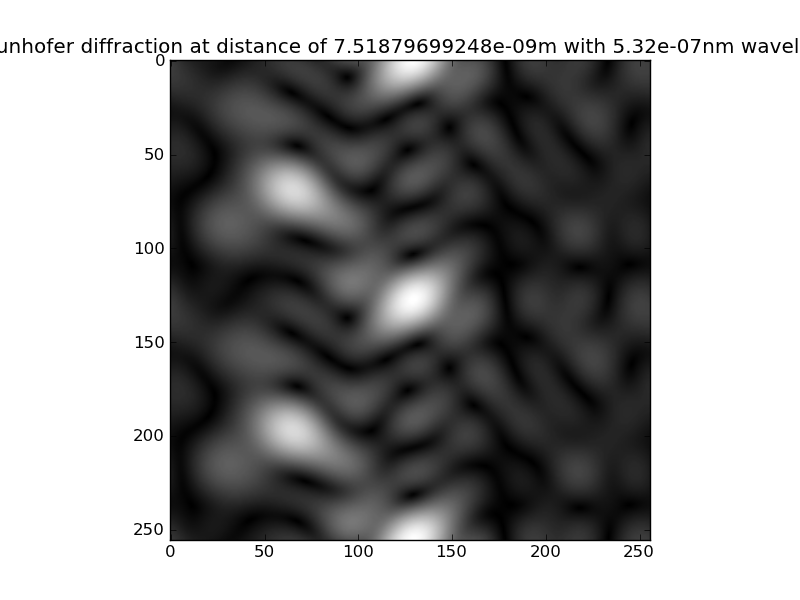
\includegraphics[width=1.9in]{q3d2}
\caption{Derived sinusoidal amplitude grating diffraction pattern.}
\label{fig:q3d2}
\end{figure}

\begin{figure}[H]
\centering
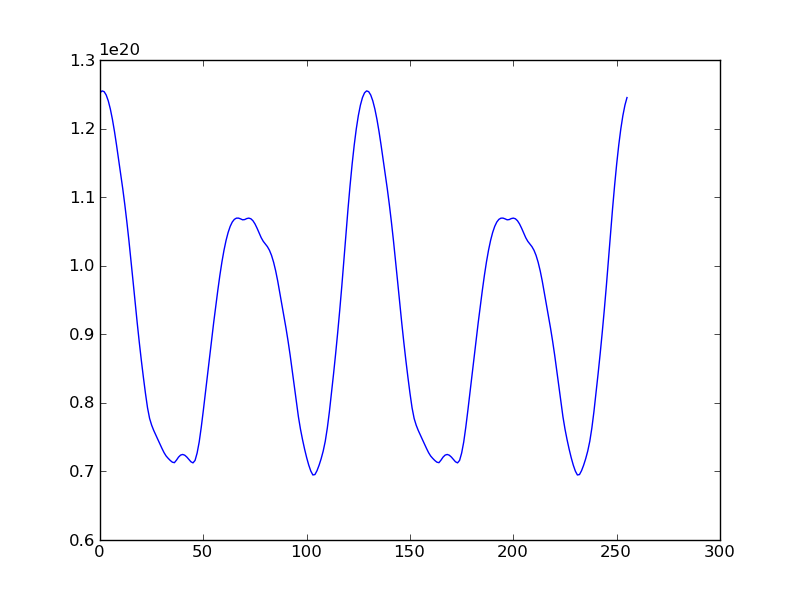
\includegraphics[width=1.9in]{q3s2}
\caption{Derived sinusoidal amplitude grating diffraction pattern cross-section.}
\label{fig:q3s2}
\end{figure}

Given patterns in above are similar to the ones in \cite{goodman2005introduction}, therefore it is verified.
\section{Conclusion}
\label{section:conclusion}
An open-source optics simulation software is presented, promoted and verified by presenting its solution to a set of known questions. The software has more items to work on it. Such as a graphical user interface and ray tracing support. In the near future it is expected to implement additional features. One can find most recent information about the discussed software under \cite{odak}. Enjoy the power of free and open-source software!

\appendices
\section{odak.py}
\label{code:odak}
\lstset{language=Python,breaklines=true}
\lstinputlisting[language=Python]{../source/lib/odak.py}

\section{sample.py}
\label{code:sample}
\lstset{language=Python,breaklines=true}
\lstinputlisting[language=Python]{../source/lib/sample.py}

\ifCLASSOPTIONcaptionsoff
  \newpage
\fi

\bibliographystyle{ieeetr}
\bibliography{references}
\end{document}



